\section{NỘI NĂNG - ĐỊNH LUẬT I NHIỆT ĐỘNG LỰC HỌC}
\subsection{LÝ THUYẾT TRỌNG TÂM}
\begin{tomtat}
\subsubsection{Nội năng}
\paragraph{Khái niệm nội năng}
\begin{dn}
	Nội năng của một vật là tổng động năng và thế năng tương tác của các phân tử cấu tạo nên vật. Nội năng của vật phụ thuộc vào nhiệt độ $T$ và thể tích $V$ của vật:
	$$U=f\left(T, V\right).$$
\end{dn}
Đơn vị của nội năng trong hệ SI là joule $\left(\si{\joule}\right)$.
\paragraph{Mối liên hệ giữa nội năng và năng lượng của các phân tử cấu tạo nên vật}
\begin{boxdn}
	Khi năng lượng của các phân tử cấu tạo nên vật tăng thì nội năng của vật tăng và ngược lại.
\end{boxdn}
\subsubsection{Các cách làm thay đổi nội năng}
\paragraph{Thực hiện công}
\begin{boxdn}
	Quá trình thực hiện công làm cho nội năng của hệ thay đổi, hệ nhận công thì nội năng của hệ tăng, hệ thực hiện công cho vật khác thì nội năng giảm.
\end{boxdn}
	\textbf{\textit{Ví dụ 1:}} Dùng tay ấn mạnh và nhanh piston của một cylanh chứa khí, thể tích khí trong cylanh giảm xuống (thế năng tương tác giữa các phân tử khí tăng), đồng thời khí nóng lên (động năng chuyển động nhiệt của các phân tử khí tăng). Do đó, nội năng của khí tăng.\\
	\textbf{\textit{Ví dụ 2:}} Chà xát hai thanh gỗ với nhau, bề mặt tiếp xúc của hai thanh gỗ nóng dần lên. Nội năng của thanh gỗ tăng.
\begin{center}
	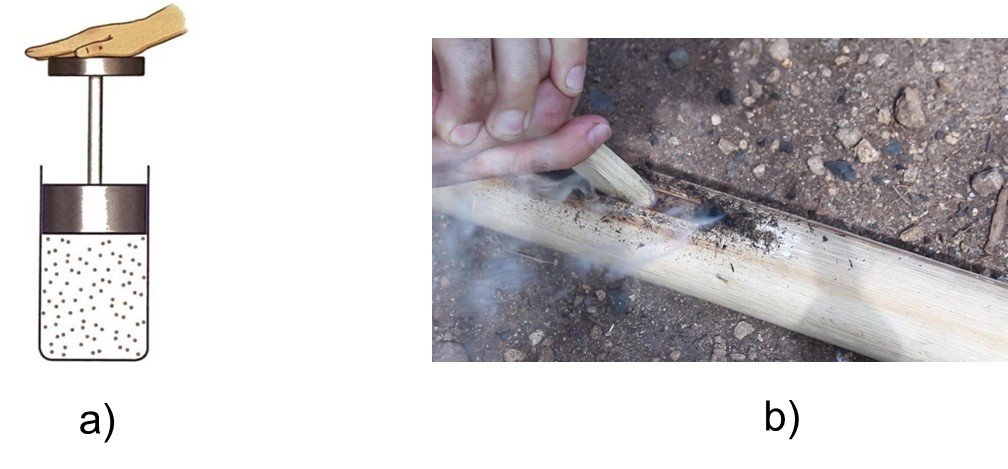
\includegraphics[width=0.45\linewidth	]{figs/VN12-Y24-PH-SYL-003-1}
	\captionof{figure}{a) Nén khối khí trong cylanh; b) Chà xát hai thanh gỗ với nhau}
\end{center}
\paragraph{Truyền nhiệt}
\begin{boxdn}
	Quá trình làm thay đổi nội năng của vật bằng cách cho nó tiếp xúc với vật khác khi có sự chênh lệch nhiệt độ giữa chúng gọi là sự truyền nhiệt.
\end{boxdn}
	\textbf{\textit{Ví dụ:}} Miếng sắt sau khi tôi luyện được thả vào chậu nước để làm nguội đi. Khi đó, nước nhận nhiệt lượng từ miếng sắt nên nội năng tăng (nhiệt độ tăng) và miếng sắt truyền nhiệt lượng cho nước nên nội năng giảm (nhiệt độ giảm).
\begin{center}
	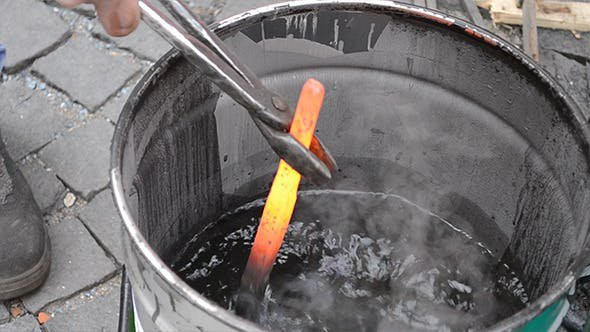
\includegraphics[width=0.3\linewidth]{figs/VN12-Y24-PH-SYL-003-2}
	\captionof{figure}{Miếng sắt nung được thả vào chậu nước}
\end{center}
\subsubsection{Định luật I nhiệt động lực học}
\begin{dl}
	Độ biến thiên nội năng của hệ bằng tổng công và nhiệt lượng mà hệ nhận được:
	\begin{equation}
		\Delta U= A+Q
	\end{equation}
\end{dl}
Trong đó:
\begin{itemize}
	\item $\Delta U$: độ biến thiên nội năng của hệ, đơn vị trong hệ SI là joule $\left(\si{\joule}\right)$;
	\item $A$: công mà hệ nhận/thực hiện, đơn vị trong hệ SI là joule $\left(\si{\joule}\right)$;
	\begin{itemize}[label=+]
		\item $A>0$: hệ nhận công;
		\item $A<0$: hệ thực hiện công.
	\end{itemize}
	\item $Q$: nhiệt lượng hệ trao đổi với bên ngoài, đơn vị trong hệ SI là joule $\left(\si{\joule}\right)$;
	\begin{itemize}[label=+]
		\item $Q>0$: hệ nhận nhiệt lượng;
		\item $Q<0$: hệ truyền nhiệt lượng.
	\end{itemize}
\end{itemize}
\begin{center}
	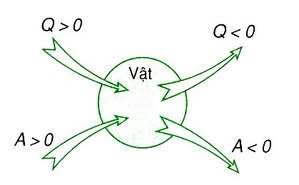
\includegraphics[width=0.35\linewidth]{figs/VN12-Y24-PH-SYL-003-3}
	\captionof{figure}{Quy ước về dấu của $Q$ và $A$}
\end{center}
\end{tomtat}
\subsection{VÍ DỤ MINH HOẠ}
\begin{dang}{Trình bày được các cách làm thay đổi nội năng}
	
\end{dang}
		\begin{vd}
		Dựa vào mô hình động học phân tử, hãy giải thích hiện tượng quả bóng bàn bị móp (nhưng chưa bị thủng) khi thả vào cốc nước nóng sẽ phồng trở lại.
			\begin{center}
				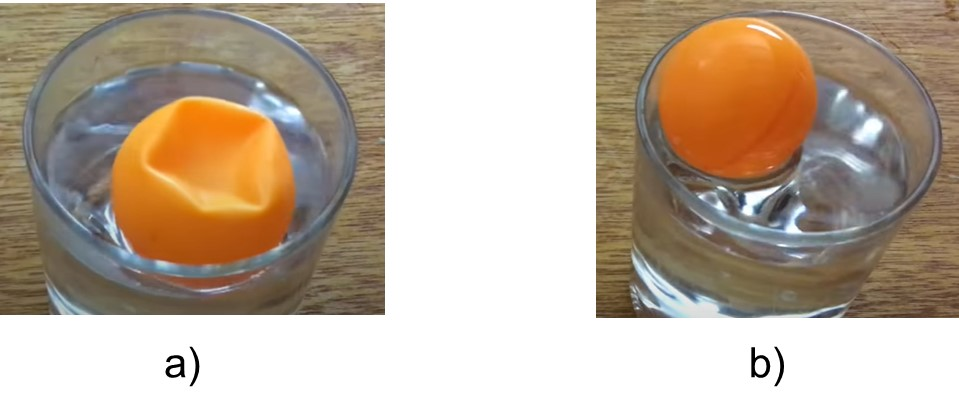
\includegraphics[width=0.45\linewidth]{{figs/VN12-Y24-PH-SYL-003-4}}
				\captionof{figure}{a) Quả bóng bàn ban đầu bị móp; b) Quả bóng sau khi được ngâm vào cốc nước nóng}
			\end{center}
			\loigiai{
				Khi thả quả bóng bi móp vào nước nóng, nhiệt độ khí trong quả bóng tăng làm các phân tử khí chuyển động nhiệt nhanh hơn nên va chạm với thành bóng nhiều hơn và mạnh hơn. Khi đó, áp suất khí trong quả bóng tăng lên và tạo ra lực đẩy đủ lớn làm vỏ cao su của quả bóng phồng trở lại}
	\end{vd}
		
		\begin{vd}
			Vì sao pha nước chanh bằng nước ấm thì đường sẽ tan nhanh hơn khi pha bằng nước lạnh? Em còn cách làm nào khác để đường tan nhanh hơn không? Hãy đưa ra lời giải thích cho cách làm của em.
			\loigiai{Khi nhiệt độ càng cao thì động năng chuyển động nhiệt của các phân tử nước và phân tử đường càng lớn. Do đó, các phân tử đường dễ dàng hoà tan vào trong nước.\\
				Để đường tan nhanh vào nước ta có thể khuấy mạnh vào nước. Khi đó, hệ nước và đường nhận công nên động năng chuyển động của các phân tử đường và nước tăng. Các phân tử đường dễ hoà tan vào nước}
		\end{vd}
	\begin{dang}{Vận dụng định luật I nhiệt động lực học}
		\end{dang}
		\begin{vd}
			Giả sử cung cấp cho hệ nhiệt động một công là $\SI{200}{\joule}$ nhưng nhiệt lượng mà hệ bị thất thoát ra ngoài môi trường là $\SI{120}{\joule}$. Hỏi nội năng của hệ tăng hay giảm bao nhiêu?
			\loigiai{Hệ nhận công nên $A>0\Rightarrow A=\SI{200}{\joule}$.\\
				Hệ toả nhiệt ra ngoài môi trường nên $Q<0\Rightarrow Q=\SI{-120}{\joule}$.\\
				Độ biến thiên nội năng của hệ:
				$$\Delta U= Q+A=\SI{80}{\joule}.$$
				Vậy nội năng của hệ tăng $\SI{80}{\joule}.$}
		\end{vd}
		\begin{vd}
		Cung cấp nhiệt lượng $\SI{1.5}{\joule}$ cho một khối khí trong một cylanh đặt nằm ngang trong chân không. Chất khí nở ra, đẩy piston đi một đoạn $\SI{5}{\centi\meter}$. Biết lực ma sát trượt giữa piston và cylanh có độ lớn là $\SI{20}{\newton}$, coi piston chuyển động thẳng đều. Tính
		\begin{enumerate}[label=\alph*)]
			\item Công của khối khí thực hiện.
			\item Độ biến thiên nội năng của khối khí.
		\end{enumerate}
		\loigiai{
			\begin{enumerate}[label=\alph*)]
				\item Do piston chuyển động thẳng đều nên lực đẩy $\vec{F}$ của khối khí tác dụng lên lên piston cân bằng với lực ma sát giữa piston và cylanh.\\
				Độ lớn công của khối khí thực hiện là:
				$$A'=F\cdot d=F_\text{ms}\cdot d=\left(\SI{20}{\newton}\right)\cdot\left(\SI{0.05}{\meter}\right)=\SI{1}{\joule}.$$
				\item Vì khối khí thực hiện công nên $A<0$: $A=-A'=\SI{-1}{\joule}$.\\
				Khối khí nhận nhiệt nên $Q>0\Rightarrow Q=\SI{1.5}{\joule}$.\\
				Độ biến thiên nội năng của khối khí:
				$$\Delta U=Q+A=\SI{1.5}{\joule}-\SI{1}{\joule}=\SI{0.5}{\joule}.$$
				Vậy nội năng của khối khí tăng $\SI{0.5}{\joule}$.
		\end{enumerate}}
		\end{vd}
		
		\begin{vd}
			Khi truyền nhiệt lượng $Q$ cho khối khí trong một cylanh hình trụ thì khí dãn nở đẩy piston làm thể tích của khối khí tăng thêm 7 lít. Biết áp suất của khối khí là $\SI{3E5}{\pascal}$ và không đổi trong quá trình khí dãn nở. Tính
			\begin{enumerate}[label=\alph*)]
				\item Công mà khối khí thực hiện.
				\item Nhiệt lượng cung cấp cho khối khí. Biết rằng trong quá trình này, nội năng của khối khí giảm $\SI{1100}{\joule}$.
			\end{enumerate}
		\loigiai{
			\begin{enumerate}[label=\alph*)]
				\item Độ lớn công khối khí thực hiện:
				$$A'=F\cdot d=p\cdot S\cdot d=p\cdot\Delta V=\left(\SI{3E5}{\pascal}\right)\cdot\left(\SI{7E-3}{\meter^3}\right)=\SI{2100}{\joule}.$$
				\item Vì khối khí thực hiện công nên $A<0$: $A=-A'=\SI{-2100}{\joule}$.\\
				Nội năng của khí giảm nên $\Delta U<0\Rightarrow \Delta U=\SI{-1100}{\joule}$.\\
				Áp dụng định luật I nhiệt động lực học, nhiệt lượng cần cung cấp cho khối khí:
				$$Q=\Delta U - A=\SI{-1100}{\joule}+\SI{2100}{\joule}=\SI{1000}{\joule}.$$
			\end{enumerate}
		}
		\end{vd}
	\subsection{BÀI TẬP TRẮC NGHIỆM}
	\Opensolutionfile{ans}[ans/G12Y24B3TN]
	\begin{ex}
		Khi nhiệt độ của vật tăng lên thì
		\choice
		{\True động năng của các phân tử cấu tạo nên vật tăng}
		{động năng của các phân tử cấu tạo nên vật giảm}
		{nội năng của vật tăng}
		{thế năng của các phân tử cấu tạo nên vật tăng}
		\loigiai{ }
		\end{ex}
% ==================================================================================
	\begin{ex}
Nội năng của một hệ là 
	\choice
	{\True tổng động năng chuyển động nhiệt và thế năng tương tác giữa các phân tử cấu tạo nên hệ}
	{tổng của động năng và thế năng của hệ}
	{tổng động năng chuyển động của các phân tử cấu tạo nên hệ}
	{tổng động lượng chuyển động hỗn loạn và thế năng tương tác giữa các phân tử cấu tạo nên hệ}
	\loigiai{ }
\end{ex}
% ==================================================================================
	\begin{ex}
	Nội năng của một hệ phụ thuộc vào
	\choice
	{nhiệt độ của hệ}
	{thể tích của hệ}
	{\True nhiệt độ và thể tích của hệ}
	{nhiệt độ, thể tích và khối lượng của hệ}
	\loigiai{ }
\end{ex}
% ==================================================================================
	\begin{ex}
Cách làm thay đổi nội năng của hệ bằng hình thức thực hiện công là
	\choice
	{bỏ thỏi sắt vào nước nóng}
	{\True chà sát miếng kim loại bằng giấy nhám}
	{đưa một thỏi sắt lên cao}
	{hơ thỏi sắt bằng đèn cồn}
	\loigiai{ }
\end{ex}
% ==================================================================================
	\begin{ex}
Khi ấn piston để nén khí trong một cylanh thì
	\choice
	{kích thước mỗi phân tử khí giảm}
	{\True khoảng cách giữa các phân tử khí giảm}
	{khối lượng mỗi phân tử khí giảm}
	{số phân tử khí giảm}
	\loigiai{ }
\end{ex}
% ==================================================================================
	\begin{ex}
	Định luật I của nhiệt động lực học là vận dụng định luật nào sau đây?
	\choice
	{Định luật bảo toàn động lượng}
	{Định luật bảo toàn cơ năng}
	{\True Định luật bảo toàn và chuyển hoá năng lượng}
	{Các định luật Newton về chuyển động}
	\loigiai{ }
\end{ex}

% ==================================================================================
	\begin{ex}
			Hệ thức $\Delta U=Q+A$ khi $Q>0$ và $A<0$ mô tả quá trình
		\choice
		{hệ truyền nhiệt và sinh công}
		{\True hệ nhận nhiệt và sinh công}
		{hệ truyền nhiệt và nhận công}
		{hệ nhận nhiệt và nhận công}
		\loigiai{ }
	\end{ex}
% ==================================================================================
		\begin{ex}
			Dùng tay nén piston và đồng thời nung nóng khối khí trong cylanh. Xác định dấu của $Q$ và $A$ của khối khí trong biểu thức của định luật I nhiệt động lực học $\Delta U=Q+A$.
		\choice
		{\True $A>0$; $Q>0$}
		{$A<0$; $Q>0$}
		{$A>0$; $Q<0$}
		{$A<0$; $Q<0$}
		\loigiai{ }
	\end{ex}
	% ==================================================================================
		\begin{ex}
		Chọn phát biểu \textbf{đúng nhất}.
	\choice
	{Động cơ nhiệt là động cơ trong đó toàn bộ phần năng lượng của nhiên liệu bị đốt cháy chuyển hoá thành cơ năng}
	{Động cơ nhiệt là động cơ trong đó một phần năng lượng của nhiên liệu bị đốt cháy chuyển hoá thành nhiệt năng}
	{\True Động cơ nhiệt là động cơ trong đó một phần năng lượng của nhiên liệu bị đốt cháy chuyển hoá thành cơ năng}
	{Động cơ nhiệt là động cơ trong đó toàn bộ năng lượng của nhiên liệu bị đốt cháy chuyển hoá thành nhiệt năng}
	\loigiai{ }
\end{ex}
% ==================================================================================

	\begin{ex}
	Khi thả một thỏi kim loại đã được nung nóng vào một chậu nước lạnh thì nội năng của thỏi kim loại và của nước thay đổi như thế nào?
	\choice
	{Nội năng của thỏi kim loại và của nước đều tăng}
	{Nội năng của thỏi kim loại và của nước đều giảm}
	{\True Nội năng của thỏi kim loại giảm, nội năng của nước tăng}
	{Nội năng của thỏi kim loại tăng, nội năng của nước giảm}
	\loigiai{ }
\end{ex}
% ==================================================================================
	\begin{ex}
	Khi ôtô đóng kín cửa để ngoài trời nắng nóng, nhiệt độ không khí trong xe tăng rất cao so với nhiệt độ bên ngoài, làm giảm tuổi thọ các thiết bị trong xe. Nguyên nhân gây ra sự tăng nhiệt độ này là do thể tích khối khí trong ôtô
	\choice
	{thay đổi nên nhiệt lượng mà khối khí trong ôtô nhận được chủ yếu làm tăng nội năng của khối khí}
	{không đổi nên nhiệt lượng mà khối khí trong ôtô nhận được chủ yếu làm giảm nội năng của khối khí}
	{thay đổi nên nhiệt lượng mà khối khí trong ôtô nhận được chủ yếu làm tăng nội giảm của khối khí}
	{không đổi nên nhiệt lượng mà khối khí trong ôtô nhận được chủ yếu làm tăng nội năng của khối khí}
	\loigiai{ }
\end{ex}
% ==================================================================================
	\begin{ex}
		Người ta thực hiện công $\SI{100}{\joule}$ để nén khí trong một cylanh. Biết trong quá trình nén, khí truyền ra ngoài môi trường nhiệt lượng $\SI{20}{\joule}$. Độ biến thiên nội năng của khí là 
		\choice
		{\True $\SI{80}{\joule}$}
		{$\SI{-80}{\joule}$}
		{$\SI{120}{\joule}$}
		{$\SI{60}{\joule}$}
		\loigiai{Khí nhận công nên $A>0\Rightarrow A=\SI{100}{\joule}$, khí toả nhiệt ra ngoài nên $Q<0\Rightarrow Q=\SI{-20}{\joule}$.\\
			Độ biến thiên nội năng của khí:
			$$\Delta U=Q+A=\SI{80}{\joule}.$$ }
	\end{ex}
% ==================================================================================
	\begin{ex}
	Khi truyền nhiệt lượng $\SI{6E6}{\joule}$ cho khí trong một cylanh hình trụ thì khí nở ra đẩy piston lên làm thể tích của khí tăng thêm $\SI{0.50}{\meter^3}$. Biết áp suất của khí là $\SI{8E6}{\newton/\meter^2}$ và coi áp suất này không đổi trong quá trình khí thực hiện công. Độ biến thiên nội năng của khí là
	\choice
	{$\SI{3E6}{\joule}$}
	{$\SI{1.5E6}{\joule}$}
	{\True $\SI{2E6}{\joule}$}
	{$\SI{3.5E6}{\joule}$}
	\loigiai{Công do khí thực hiện:
		$$A'=F\Delta x=pS\Delta x=p\Delta V=\SI{4E6}{\joule}.$$
		Vì khí thực hiện công nên $A<0\Rightarrow A=-A'=-\SI{4E6}{\joule}$.\\
		Độ biến thiên nội năng của khí:
		$$\Delta U=Q+A=\SI{2E6}{\joule}.$$}
\end{ex}
% ==================================================================================
 
\begin{ex}
Một khối khí chứa trong một cylanh đặt thẳng đứng, miệng cylanh được đậy kín bằng một piston nhẹ có tiết diện $\SI{10}{\centi\meter^2}$, có thể dịch chuyển không ma sát trong cylanh. Người ta kéo đều piston lên cao một đoạn $\SI{10}{\centi\meter}$. Biết nhiệt độ khối khí không đổi, áp suất khí quyển bằng $\SI{101325}{\pascal}$ và công do khối khí sinh ra trong quá trình này là $\SI{7.5}{\joule}$. Công cần thực hiện để kéo piston là
	\choice
	{$\SI{2.31}{\joule}$}
	{\True $\SI{2.63}{\joule}$}
	{$\SI{17.63}{\joule}$}
	{$\SI{7.5}{\joule}$}
	\loigiai{\begin{center}
			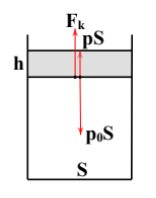
\includegraphics[width=0.25\linewidth]{figs/VN12-Y24-PH-SYL-003P-2}
		\end{center}
		Piston được nâng lên đều nên:
		$$F_k=\left(p_0-p\right)S.$$
		Công cần thực hiện:
		$$A=F_k\Delta h=\left(p_0-p\right)S\Delta h=p_0S\Delta h-A_\text{khí}=\SI{2.6325}{\joule}.$$}
\end{ex}
	\Closesolutionfile{ans}
\subsection{TRẮC NGHIỆM ĐÚNG/SAI}
\setcounter{ex}{0}
% ===================================================================
\begin{ex}
	Trong quá trình nóng chảy của vật rắn
	\choiceTF[t]
	{\True Nhiệt được truyền vào vật rắn để làm tăng nhiệt độ của nó}
	{Động năng trung bình của các phân tử trong vật rắn giảm đi}
	{Nội năng của vật rắn không thay đổi}
	{\True Tại nhiệt độ nóng chảy, nội năng không thay đổi}
	\loigiai{\begin{enumerate}[label=\alph*)]
			\item Đúng.
			\item Sai. Động năng trung bình của các phân tử trong vật rắn tăng lên.
			\item Sai. Nội năng của vật rắn thay đổi.
			\item Đúng. Nội năng không thay đổi tại nhiệt độ nóng chảy, vì năng lượng được sử dụng để làm tan chảy các liên kết giữa các phân tử mà không làm thay đổi nhiệt độ.
	\end{enumerate}}
\end{ex}
% ===================================================================
\begin{ex}
	Bố trí thí nghiệm như hình bên. Dùng đèn cồn đun nóng ống nghiệm cho đến khi nút bấc bật ra.
	\begin{center}
		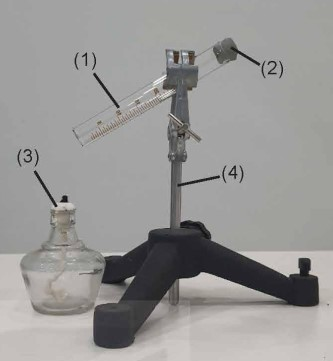
\includegraphics[width=0.3\linewidth]{figs/VN12-Y24-PH-SYL-003P-5}
	\end{center}
	\choiceTF[t]
	{Khi nút chưa bị bật ra, nội năng của không khí trong ống nghiệm không thay đổi}
	{Nội năng của không khí trong ống nghiệm tăng không chỉ do động năng chuyển động nhiệt của các phân tử khí tăng mà còn do thế năng tương tác giữa chúng tăng}
	{Nút bấc bị ra là kết quả của áp suất bên trong ống nghiệm giảm đi}
	{\True Quá trình nút bấc bật ra ngoài thì khí trong ống đang thực hiện công}
	\loigiai{\begin{enumerate}[label=\alph*)]
			\item Sai. Nội năng khí trong ống tăng do nhận nhiệt.
			\item Sai. Thế năng tương tác giữa các phân tử phụ thuộc khoảng cách giữa các phân tử, không phụ thuộc vào nhiệt độ.
			\item Sai. Nút bấc bị ra là kết quả của áp suất bên trong ống nghiệm tăng lên.
			\item Đúng.
	\end{enumerate}}
\end{ex}
% ===================================================================
\begin{ex}
	Khối khí được chứa trong cylanh, bên trên được nút kín bằng piston cách nhiệt như hình bên dưới. Dùng tay ấn mạnh piston đồng thời nung nóng bên dưới cylanh bằng ngọn lửa đèn cồn.
	\begin{center}
		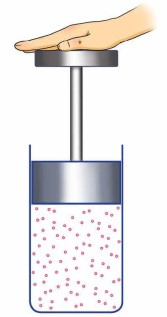
\includegraphics[width=0.15\linewidth]{figs/VN12-Y24-PH-SYL-003P-3}
	\end{center}
	\choiceTF[t]
	{\True $A>0$ vì khí nhận công (khí bị nén)}
	{$Q<0$ vì khí bị nung nóng}
	{\True Nội năng của khí trong cylanh tăng}
	{Động năng chuyển động nhiệt của các phân tử khí giảm}
	\loigiai{\begin{enumerate}[label=\alph*)]
			\item Đúng.
			\item Sai. Khí nhận nhiệt nên $Q>0$.
			\item Đúng.
			\item Sai. Động năng chuyển động nhiệt của các phân tử khí tăng.
	\end{enumerate}}
\end{ex}
% ===================================================================
\begin{ex}
	Người ta cung cấp nhiệt lượng \SI{20.6}{\joule} cho một lượng khí trong xilanh đặt nằm ngang trong chân không. Lượng khí nở ra đẩy pittông di chuyển đều đi được \SI{4}{\centi\meter}. Cho lực ma sát giữa pittông và xilanh là \SI{15}{\newton}. $Q$ và $A$ là nhiệt lượng và công mà hệ nói trên nhận từ vật khác hoặc truyền cho vật khác, $Q$ và $A$ tuân theo quy ước dấu của định luật I của nhiệt động lực học.
	\choiceTF[t]
	{\True Quá trình trên khí thực hiện công nên $A<0$}
	{Độ lớn của công mà chất khí thực hiện để pít tông chuyển động đều là \SI{60}{\joule}}
	{\True Quá trình trên hệ nhận nhiệt lượng nên $Q>0$}
	{\True Độ biến thiên nội năng của khí là \SI{20}{\joule}}
	\loigiai{
		\begin{itemchoice}
			\itemch Đúng. 
			\itemch Sai. $\left|A\right|=F_{\mathrm{ms}}\cdot s=\SI{0.6}{\joule}\Rightarrow A=\SI{-0.6}{\joule}$.
			\itemch Đúng.
			\itemch Đúng. $Q=\SI{20.6}{\joule}\Rightarrow \Delta U=Q+A=20,6-0,6=\SI{20}{\joule}$.
		\end{itemchoice}
	}
\end{ex}
\subsection{BÀI TẬP TỰ LUẬN VÀ TRẢ LỜI NGẮN}
\setcounter{ex}{0}
% ====================================================================================
\begin{ex}
	Giả sử một người đang thực hiện bài vận động vất vả chẳng hạn như nâng tạ hoặc đạp xe. Cơ thể đang thực hiện công và đồng thời nhiệt lượng thoát ra ngoài qua lỗ chân lông vào không khí xung quanh. Theo định luật I nhiệt động lực học, nhiệt độ cơ thể sẽ giảm dần trong quá trình tập luyện. Tuy nhiên, điều đó lại không xảy ra. Như vậy, có phải định luật I nhiệt động lực học không đúng trong trường hợp này phải không? Hãy giải thích.
	\loigiai{
		Trong quá trình vận động cơ thể con người thực hiện công và toả nhiệt ra ngoài môi trường nhưng trong cơ thể người luôn có năng lượng dự trữ để cung cấp năng cho các hoạt động của cơ thể. Năng lượng dự trữ này có được do các quá trình biến đổi chất dinh dưỡng từ thức ăn. Vì vậy, cơ thể luôn được duy trì ở nhiệt độ ổn định và định luật I nhiệt động lực học trong trường hợp này vẫn được nghiệm đúng.
	}
\end{ex}
% ===============================================================
\begin{ex}
	Một lượng khí nhận nhiệt lượng \SI{250}{\kilo\joule} do được đun nóng; đồng thời nhận công \SI{500}{\kilo\joule} do bị nén. Độ tăng nội năng của lượng khí là bao nhiêu \si{\kilo\joule}?
	\shortans[oly]{750}
	\loigiai{
		$\Delta U=Q+A=\SI{750}{\kilo\joule}$.
	}
\end{ex}
% ===============================================================
\begin{ex}
	Một lượng khí trong một xilanh hình trụ bị nung nóng, khí nở ra đẩy pit-tông lên làm thể tích tăng thêm \SI{0.02}{\meter^3} và nội năng tăng thêm \SI{1280}{\joule}. Biết áp suất của khối khí là \SI{2E5}{\pascal} và không đổi trong quá trình dãn nở. Nhiệt lượng đã truyền cho khí bằng bao nhiêu \si{\joule}?
	\shortans[oly]{5280}
	\loigiai{
		$A=-p\Delta V=\SI{-4000}{\joule}$.\\
		$\Delta U=Q+A\Rightarrow 1280=Q-4000\Rightarrow Q=\SI{5280}{\joule}$.
	}
\end{ex}

% ===============================================================
\begin{ex}
	Một viên đạn bằng chì có khối lượng $m=\SI{50}{\gram}$ và nhiệt dung riêng $c=\SI{0.12}{\joule/\kilogram\cdot\kelvin}$ đang bay với vận tốc \SI{360}{\kilo\meter/\hour} thì xuyên qua một tấm tấm thép mỏng, vận tốc viên đạn sau khi xuyên qua tấm thép giảm còn \SI{72}{\kilo\meter/\hour}. Tính lượng nội năng tăng thêm của hệ đạn và thép trong quá trình đạn xuyên qua thép theo đơn vị \si{\kilo\joule}.
	\shortans[oly]{0,24 }
	\loigiai{
		$\Delta t=W_{\text{đ1}}-W_{\text{đ2}}=\SI{0.24}{\kilo\joule}$.
	}
\end{ex}
% ===================================================================================
\begin{ex}
	Một quả bóng khối lượng $\SI{200}{\gram}$ rơi từ độ cao $\SI{15}{\meter}$ xuống sân và nảy lên được $\SI{10}{\meter}$. Độ biến thiên nội năng của quả bóng là bao nhiêu joule? Lấy $g=\SI{10}{\meter/\second^2}$.
	\shortans[oly]{10}
	\loigiai{
	Độ biến thiên nội năng của quả bóng:
	$$\Delta U=mg\left(h-h'\right)=\SI{10}{\joule}.$$
}
\end{ex}

% ===================================================================================
\begin{ex}
	Một vật khối lượng $\SI{1}{\kilogram}$ trượt không vận tốc đầu từ đỉnh xuống chân một mặt phẳng dài $\SI{21}{\meter}$, nghiêng $\SI{30}{\degree}$ so với mặt nằm ngang. Tốc độ của vật ở chân mặt phẳng nghiêng là $\SI{4.1}{\meter/\second}$. Tính công của lực ma sát và độ biến thiên nội năng của vật trong quá trình chuyển động trên theo đơn vị joule. Lấy $g=\SI{9.8}{\meter/\second^2}$. Bỏ qua sự trao đổi nhiệt với mặt phẳng nghiêng. Kết quả làm tròn đến chữ số hàng phần mười,
	\shortans[oly]{94,5}
	\loigiai{
		Công của lực ma sát:
		$$A_\text{ms}=W_\text{s}-W_\text{t}=mgh_\text{s}+\dfrac{1}{2}mv^2_\text{s}-mgh_\text{t}-\dfrac{1}{2}mv^2_\text{t}=\dfrac{1}{2}mv^2_\text{s}-mg\ell\sin\SI{30}{\degree}\approx\SI{-94.5}{\joule}.$$
		Độ biến thiên nội năng của vật trong quá trình chuyển động bằng công của lực ma sát:
		$$\Delta U=\SI{94.5}{\joule}.$$
	}
\end{ex}
